%\documentclass[aps,prl,twocolumn,showpacs,superscriptaddress,groupedaddress]{revtex4-1}  % for review and submission
%\documentclass[aps,preprint,showpacs,superscriptaddress,groupedaddress]{revtex4-1}  % for double-spaced preprint

%Phys Rev B
%Letter or rapid communication - 3500 words
%\documentclass[prb,groupedaddress,reprint]{revtex4-1}
%APL
\documentclass[aps,prl,twocolumn,showpacs,superscriptaddress,groupedaddress]{revtex4-1}
%\documentclass[aps,prl,reprint]{revtex4-1}
%\documentclass[aip,jap,reprint]{revtex4-1}
\usepackage[english]{babel}
\usepackage{graphicx}% Include figure files
\usepackage[pdftex,unicode,colorlinks, citecolor=blue,%
filecolor=black, linkcolor=blue, urlcolor=black]{hyperref}
\usepackage[figure,table]{hypcap} %links should lead to the begining
                                %of figure or table...

\begin{document} %Max size in pdf for APL - 4 print pages

\title{More effective than a ``super'' absorption in spherical nanoparticles}


\author{Konstantin Ladutenko} \email[e-mail: ]{fisik2000@mail.ru}
\affiliation{ITMO University, 49 Kronverskii Ave., St.~Petersburg
  197101, Russian Federation\\}

\affiliation{Ioffe Physical-Technical Institute of the Russian
  Academy of Sciences,
  26 Polytekhnicheskaya Str., St.~Petersburg 194021, Russian
  Federation}

\author{Ovidio Pe\~{n}a-Rodr\'{i}guez} \affiliation{Instituto de
  Fusi\'{o}n Nuclear, Universidad Polit\'{e}cnica de Madrid,\\
  Jos\'{e} Guti\'{e}rrez Abascal 2, E-28006 Madrid, Spain}


% \author{Pavel Belov}
% \affiliation{ITMO University, 49 Kronverskii Ave., St.~Petersburg
%   197101, Russian Federation\\}
\author{Ali Mirzaei} 
\author{Andrey Miroshnichenko}
\author{Ilya Shadrivov}
\affiliation{Nonlinear Physics Centre, Research School of Physics and Engineering,
The Australian National University, 59 Mills Rd, Acton, ACT, 2601, Australia}

\date{\today}
% APL 250 words! Phys Rev B less then 500 words, about
% 5% ot total paper length
% emacs M-x count-words

\begin{abstract}
  There is a theoretical limit for absorption by a sub-wavelength bulk
  spherical particle.  To overcome this limit we applied a widely used
  ``super'' design pattern which superpose several electric and
  magnetic multipole resonances of a multilayered particle.  We used a
  straightforward approach to evaluate a number of designs from realistic
  materials.  However, we found that due to dimension effect it can be
  preferable to use a properly designed smaller particle with only a
  dipole response in order to reach the best absorption efficiency.
\end{abstract}


\pacs% insert suggested PACS numbers in braces on next line
{41.20.Jb 42.25.Bs 02.60.Pn 02.70.-c}
%41.20.Jb	Electromagnetic wave propagation
%42.25.Bs       Wave propagation, transmission and absorption
%%42.25.Fx	Diffraction and scattering
%02.60.Pn	Numerical optimization
%02.70.-c	Computational techniques; simulations 

\maketitle %\maketitle must follow title, authors, abstract and \pacs

Mie theory~\cite{Mie-1908} describes interaction of an electromagnetic
wave with a spherical particle.  In spite of its long history lasting
over a century it is still of great interest our
days~\cite{Suzuki-2008,MacKowski-2012,Lerme-2000,Xu-2005,Li-2006,Gogoi-2010,Santiago-2011}.
Development of Mie theory~\cite{Yang-2003, Pena-scattnlay-2009} made
it possible to explore properties of multilayered spherical
particles~\cite{Sheehan-2013,Selmke-2012}. Such particles has various
applications in cancer treatment~\cite{Zhang-2010, Hirsch-2003} and
medical diagnostics~\cite{Allain-2002},
cloaking~\cite{Qui-2009,Semouchkina-2013, Ladutenko-2014} and
plasmonic~\cite{Martin-2013, Alu-2005} devices, study on thermal
properties of insulating material~\cite{Xie-2013}, solar cells\cite{Kameya-2011,Mann-2011},
and so on.

The problem of scattering from a multilayered cylinder and a sphere
was investigated in great detail with Fan~et~al.~\cite{Fan-2010,Fan-2011}.
In his work he defined a ``super'' scatterer as a sub-wavelength object
having a scattering cross section that far exceeds the single-channel
limit of the maximal total angular momentum involved.  From spectral
point of view this means the superposition of several electric and/or
magnetic resonances.

There is a similar problem to design highly absorbing sub-wavelength
particles.  Tribelsky has derived~\cite{Tribelsky-2011} a theoretical
limit of a maximum absorption value for a single channel.  As a result
the absorption coefficients $\tilde{a}_n= {\rm Re}\{a_n\} - |a_n|^2 $
and $\tilde{b}_n= {\rm Re}\{b_n\} - |b_n|^2 $ become limited with
$1/4$ in case of largest possible absorption (where $a_n$ and $b_n$
are scattering coefficient as defined in Mie
theory~\cite{Bohren-1983}.  To overcome a single-channel limit we
tried to use similar approach and to tune together several absorption
resonances.

We used a triple layered $Si/Ag/Si$ spherical particle with
experimental material parameters from Palik~\cite{palik-1997}
illuminated with a plane wave~(Fig. TODO ).  To optimize width of each
layer we implemented~\cite{JADE-web} adaptive differential
evolution~\cite{Storn-DE-first-1997} algorithm named
JADE~\cite{Jingqiao-JADE-2009}.  All the details on the optimization
procedure can be found elsewhere~\cite{Ladutenko-2014}.  Mie
calculations were performed with the
Scattnlay~\cite{Pena-scattnlay-2009,Scattnlay-web} software, whose results were
verified against a number of other Mie-type codes and commercially
available programs Comsol Multiphysics~\cite{CST-web} and CST Microwave
studio~\cite{CST-web}.

Initially we tried to maximize contribution of several multipole
resonances at a given wavelength $\lambda=500$~nm.  However, best
results were obtained with the optimizer set to find maximum of the
absorption efficiency factor $Q_{\rm abs}=C_{\rm abs}/2\pi R_{\rm
  total}^2$, where $R_{\rm total}$ is the outer radius of the particle
and $C_{\rm abs}$ denotes its absorption cross-section.  This way, the
efficiency is defined as absorption cross-section normalized to the
geometrical cross-section of the particle. 

\begin{figure}
  \center{
    % Use pdfcrop to remove white margins
    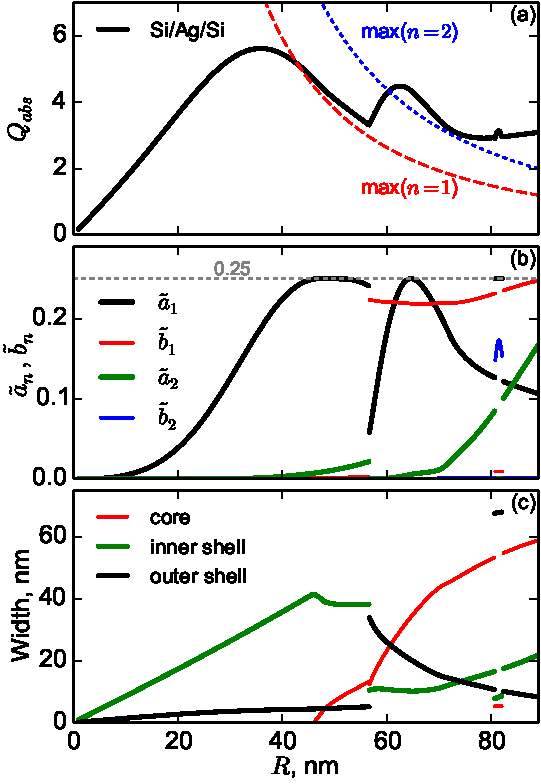
\includegraphics[width=0.4\textwidth]{fig/2015-04-01-Qabs-SiAgSi-overview}%
    \caption{ Optimized designs overview at working wavelength
      $\lambda = 500$~nm. (a) Scattering
      coefficients (b) Absorption efficiency with best value at total
      R=36~nm and Ag/Si design (zero sized core) and ``super'' designs
      at R=63~nm and R=81~nm. (c) Used layers width, for total
      $R<46$~nm the core width was optimized to be zero, the design
      become bi-layer $Ag/Si$ particle. 
      \label{fig:overview}
    }%
  }
\end{figure}
In order to understand the phenomena we run a series of optimizations;
we were steadily increasing the outer size of the particle starting
from zero.  The dependence of highest absorption efficiency obtained
with the optimization procedure on the spherical particle outer radius
is depicted in Fig.~\ref{fig:overview}a.  With dashed lines we marked
the absorption limit of dipole ($n=1$) and quadrupole ($n=2$) resonances
derived with Tribelsky~\cite{Tribelsky-2011} as $$Q^{(n)}_{\rm abs\
  max}=\frac{2n+1}{2q^2},$$ where size parameter $q=2\pi R_{\rm
  total}/\lambda$.  This limits are obviously beaten for $R_{\rm
  total}>60$~nm, as far as the contribution of higher multipoles with
$n>2$ in negligible for the plotted range of outer size of the
particle.  All this designs should be classified as ``super''
absorbers as it follows from the Fan~et~al.~\cite{Fan-2010,Fan-2011}
definition.

In Fig.~\ref{fig:overview}b we present values of absorption
coefficients; horizontal dashed line denotes their theoretical limit.
For small particles the absorption is dominated with electric dipole
$\tilde{a}_1$.  At $R_{\rm total} = 56.6$~nm the optimizer switches to
the branch of designs, that combine the usage of electric and magnetic
dipoles, as far as they start to outperform the single electric dipole
designs branch.  There is one more branch of designs using electric
dipole $\tilde{a}_1$ and magnetic quadrupole $\tilde{b}_2$, however,
it turns to be the best in a very limited range of $R_{\rm total}$ from
80.7~nm to 82.1~nm.

Fig.~\ref{fig:overview}c unveils the fact of dipole design branch has
two parts. For $R_{\rm total}<46$~nm the optimizer nullifies the
innermost layers width (marked as a ``core'' layer); the particle
design was reduces to $Ag/Si$ bi-layer.  At $R_{\rm total}=46$ dipole
channel becomes practically indistinguishable from the theoretical
limit (it becomes $\tilde{a}_1>0.249$).  It looks like the optimizer
introduced the inner $Si$ layer in order to keep $\tilde{a}_1$ near
the theoretical limit as the $R_{\rm total}$ increases further on.  As
a side effect quadrupole $\tilde{a}_2$ appears, however, it do not
help to reach ``super'' absorption limit $n=2$.

The most important feature of Fig.~\ref{fig:overview} is that the best
absorption efficiency was reached in non ``super'' absorption mode;
even more, it was reached before $\tilde{a}_1$ hit the single channel
limit.  This way to achieve the best absorption efficiency there is no
need to tune several multipole resonances using complex multilayer
structure.  From practical point of view it is even more important that
the maxima can be reached in bi-layer structure, instead of
triple-layer; it should be easier (and cheaper) to produce such an
absorber.

\begin{figure}
  \center{
    % Use pdfcrop to remove white margins
    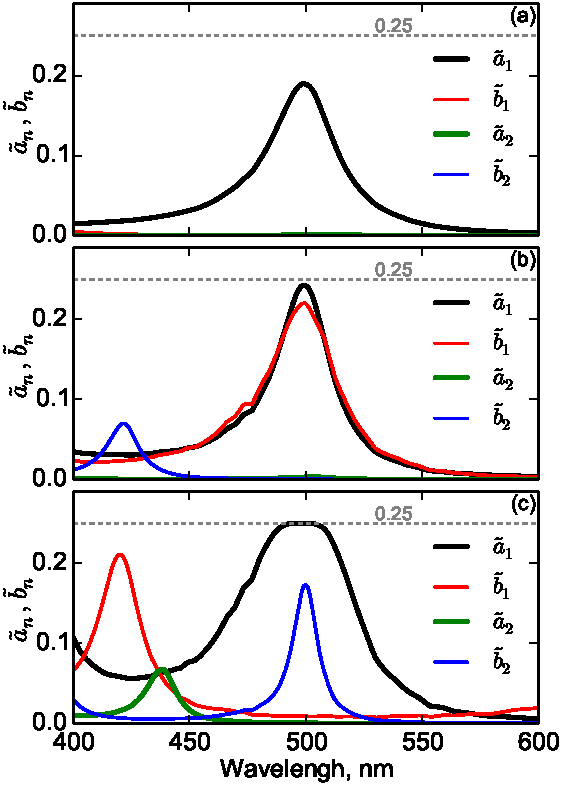
\includegraphics[width=0.4\textwidth]{fig/2015-04-01-SiAgSi-ab-spectra3.pdf}%
    \caption{Expansion coefficients spectra of (a) efficient and (b-c)
      ``super'' design.      
      \label{fig:spectra}
    }%
  }
\end{figure}
To verify large absorption coefficient obtained during optimization
corresponds to a multipole resonance we plotted in
Fig.~\ref{fig:spectra} spectra of absorption coefficients for all
designs that have a local maxima of $Q_{\rm abs}$ on
Fig.~\ref{fig:overview}a.  As expected design with maxima at R=36~nm
has a single electric dipole resonance with the center at optimized
wavelength $\lambda=500$~nm.  Spectra of designs with maximum at
R=63~nm and R=81~nm has a ``super'' structure; there is a
superposition of electric and magnetic resonances.  These spectra also
has some other resonances, however, they are located rather far from
the used wavelength.  A noticeable feature of Fig.~\ref{fig:spectra}c is
an almost flat top of the electric dipole resonance. (TODO add some
explanation, why it flat? Any ideas?)

\begin{figure}
  \center{
    % Use pdfcrop to remove white margins
    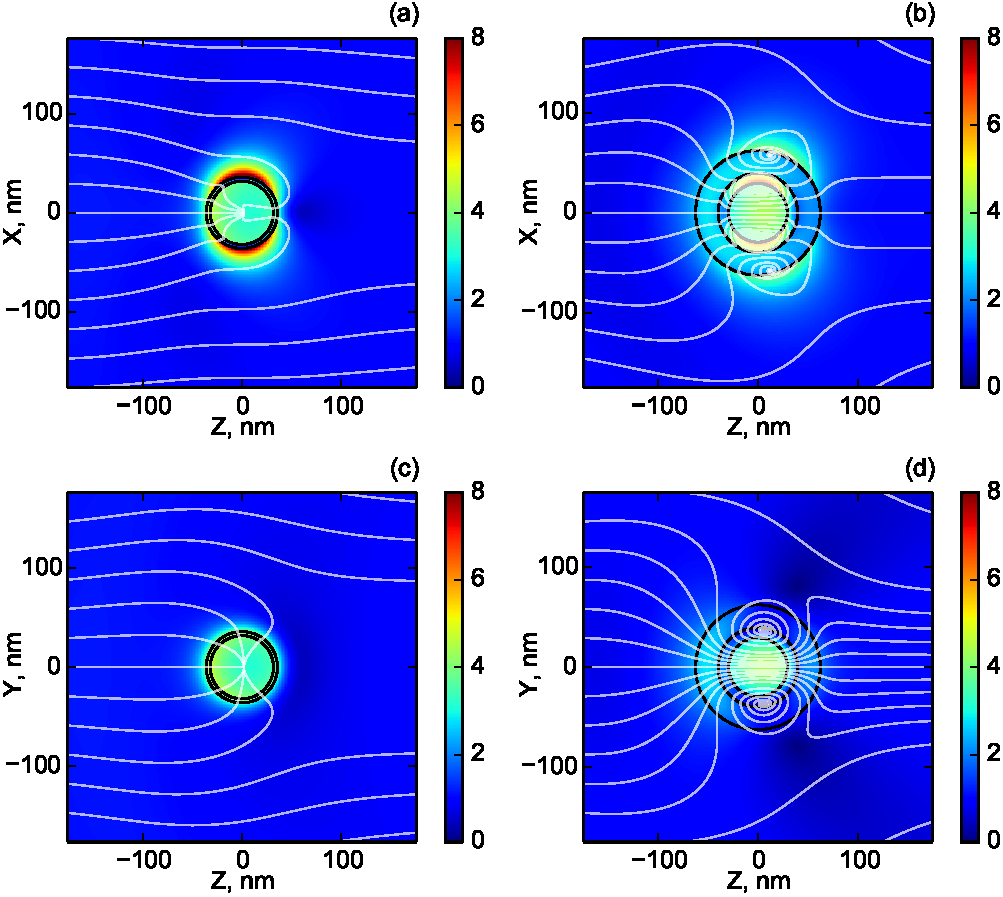
\includegraphics[width=0.4\textwidth]{fig/SiAgSi-flow-R62-YZ-Eabs.pdf}%
    \caption{ Amplitude of electric field for efficient (a,c) and
      ``super'' (b,d) designs in E-k  (a-b) and H-k (c-d) planes. 
      \label{fig:field}
    }%
  }
\end{figure}
Finally, we present distribution for amplitude of electric field
(Fig.~\ref{fig:field}) for two designs: with the best efficiency and a
``super'' absorber.  We set different scale for this two designs so
that black circles that denote outer boundary are plotted to be the
same size.  We also plot streamlines for a Poynting vector, the last
one is tangent at each point to the white curve.  For the effective
design the power flow goes into the particle.  In case of ``super''
absorption presence of the magnetic response leads to the existence of
power flow vortexes, there is some power leaking throw the particle.









% . Our initial idea was to show the
%   same effect in absorption, and R=63 with R=81nm are such
%   `superabsopting` designs. However, in 3D case (in contrast to 2D
%   investigated with Ali) it turned out that sometimes it is preferable
%   to use a smaller particle with single resonance to achieve the best
%   efficiency. This way, in 3D case using real materials for a
%   multilayer spherical particle ``superabsorbing'' design do not
%   always leads to best absorption efficiency. Moreover, same effect
%   exists for scattering from SiAgSi optimized structure. At WL=500 nm
%   ``super'' scattering mode with two resonances gives the best
%   efficiency, however, at WL=400 nm a single resonance small particle
%   has a better scattering efficiency compared to larger particles with
%   ``super'' design.







% \begin{acknowledgments}
%   The authors would like to thank the Ministry of Education and
%   Science of the Russian Federation (Goszadanie 2014/190, Zadanie
%   No. 3.561.2014/K, project 14.584.21.0009 10), Russian Foundation for Basic
%   Research (Grant 15-02-01344), and Government of the Russian
%   Federation (Grant 074-U01) for the financial support. The
%   simulations of cloak designs has been funded by the Russian Science
%   Foundation Grant No. 14-12-01227.% We
%   % would also like to appreciate Alexander Krasnok for the help with
%   % CST simulations and Ilya V. Shadrivov for valuable comments on the
%   % manuscript.
% \end{acknowledgments}

This way we conclude, that to design a good absorber it is not
necessary to superpose several resonances.  The explanation for the
phenomena seems to be quite intuitive.  Due to spatial structure of
higher multipoles, namely presence of nodal point, they are not using
effectively the whole volume of the particle for the absorption. At
the same time in 3D the increased absorption of higher multipoles should
compete against quadratic growth of the geometrical cross-section.  It
is clearly not the point for the case under consideration, the most
effective design has simply the smallest radius.


It is interesting, that similar conclusion was made by Miller et
al~\cite{Miller-2014} for extinction of arbitrary particles.


\bibliography{2015-Ladutenko-Qabs}
\end{document}

